\documentclass[final,twocolumn]{elsarticle}
\usepackage{booktabs}
\usepackage[hyphens]{url}
\usepackage[usenames,dvipsnames]{color}
\usepackage{comment}
\usepackage{float}
\usepackage{lipsum}
\usepackage{pifont}
 \usepackage[english]{babel}
\usepackage{array}
\usepackage{multirow}
\usepackage{amssymb}
\usepackage{amsthm}
\usepackage{amsmath}
\usepackage[normalem]{ulem}
\usepackage{xspace}
\usepackage{datetime}
\usepackage{hyperref}

% *** GRAPHICS RELATED PACKAGES ***
%
% \usepackage[pdftex]{graphicx}
% declare the path(s) where your graphic files are
\graphicspath{{./images/}}
% and their extensions so you won't have to specify these with
% every instance of \includegraphics
\DeclareGraphicsExtensions{.pdf,.jpeg,.png}

\usepackage{etoolbox}
\makeatletter
\patchcmd{\@makecaption}
  {\scshape}
  {}
  {}
  {}
\makeatother

\usepackage[font=footnotesize,labelfont=bf]{caption}
\captionsetup{justification=raggedright,singlelinecheck=false}

\hyphenation{WEB-rick op-tical net-works semi-conduc-tor}
\newcommand{\CRASH}{{\sc \{CrashSim\}}\xspace}
\hypersetup{%
%  pdftitle = {\CRASH: Catching the Unexpected},
  pdftitle = {Charting a Course Through Uncertain Environments: SEA Uses Past Problems to Avoid Future Failures}
  pdfkeywords = {},
  pdfauthor = {Preston Moore, Justin Cappos, Phyllis Frankl, Thomas Wies},
  bookmarksnumbered,
  bookmarksopen=true,
  colorlinks=true,
  urlcolor=[rgb]{.35,0,0},
  linkcolor=[rgb]{.35,0,0},
  citecolor=[rgb]{.35,0,0},
  pdfstartview={FitH},
}

\input{annotations}

\newcommand{\tickmark}{\ding{51}}
\newcommand{\xmark}{\ding{55}}

\begin{document}

\begin{frontmatter}

\title{Charting a Course Through Uncertain Environments: SEA Uses Past Problems to Avoid Future Failures}

% author names and affiliations
% use a multiple column layout for up to three different
% affiliations
\address[add1]{New York University: Tandon School of Engineering}
\address[add2]{New York University: Courant Institute of Mathematical
  Sciences}
\author[add1]{Preston Moore}
\ead{pkm266@nyu.edu}
\author[add1]{Justin Cappos}
\ead{jcappos@nyu.edu}
\author[add1]{Phyllis Frankl}
\ead{pfrankl@nyu.edu}
\author[add2]{Thomas Wies}
\ead{wies@cs.nyu.edu}

\input{abstract}

\end{frontmatter}

\input{introduction}
\section{What is an Environment?}
\label{SEC:background}

It is important
to have a clear understanding
of what constitutes an application's environment
in order to see how it can contribute to the presence of bugs.
An application's environment consists of
all of the components an application depends upon
that its developers do not control.
In practice, this is everything other than the code and data packaged
within the application itself.
Typically testers
focus on explicit inputs to the application
and overlook the implicit inputs
coming from these uncontrolled components.

Anything external to the application can be
configured in unexpected ways.
For example, library search rules can result in default system libraries
being loaded instead of
the versions deployed alongside the application.
These external resources can be thought of as
providing implicit inputs to the program that affect its flow of execution.
An investigation of bug reports has shown that environmental bugs in the
following categories have been found in major applications.

\begin{itemize}

\item {\bf Operating Systems.} Differences in the way operating systems
implement system calls can influence the behavior of applications.  For
example, on Linux it is possible to remove an open file, yet this is not
allowed on Windows systems~\cite{UnlinkStandard}.  An application
written without this difference in mind could fail if it relies on one
implementation or the other.

\item {\bf File Systems.}  The exact file system used will also have a
substantial impact on the behavior of a system, independent of the
operating system.  The popular Ext4 file system on Linux is case sensitive,
so that ``a'' and ``A'' are different files,
while in OS X's HFS+ file system
those file names would refer to the same file.
File systems can have varying limits or behaviors for other items as well,
including file name length (popularized due to the 8.3 limitations of the
FAT file system), maximum file length, number of directory entries, or
depth
of directories supported, all of which can lead to errors when programs
do not account for these variations~\cite{EXT4Layout, AppleHFS}.
The layout and contents of a filesystem can also impact an application's
execution.  Unexpected file types can result in application
failures, and multi-disk layouts impose additional requirements on
common operations, such as moving a file from one location to
another.
        We explore the latter two situations in our
        evaluation (Sec.~\ref{sec-env-bugs}).

\item {\bf Network.} Both local and remote network nodes
can have specific characteristics that could influence the behavior of an
application.
For example, POSIX operating
systems support the notion of limiting the kernel buffer set aside for a
socket.  However, many other popular operating
systems (Windows, Linux, and Mac)
implement this quite differently.
If a UDP datagram
larger than the specified buffer size is received by a Linux system,
it will be dropped.
Windows,
however,
will receive these datagrams,
but it will influence data retrieval.
Any system calls that retrieve data from the buffer in which
datagrams are
stored will only return a number of bytes less than or equal to the
buffer size, requiring multiple calls
to retrieve all the data.~\cite{Zhuang_NSDI_2014}.

\item {\bf Processor.}  The processor used can also influence the
behavior of an application.  This is frequently
evidenced through the different floating point behaviors a
processor may exhibit~\cite{ArbitraryPrecision}.
In addition, bugs are fairly common
in processors and will cause variances, as will
differences in interpreting
how to execute complex instructions~\cite{Microarch}.

\end{itemize}

In this work, we chose to focus on operating system,
file system, and network
environmental issues.
These issues are
readily visible in data returned
by the system calls
an application makes.
We took advantage of this in our implementation of SEA as CrashSimulator by
intercepting and manipulating system call results.
As we will discuss, this allowed us to strike a good balance between a
higher level approach, such as hooking library functions, and a lower level
approach like directly altering memory values.
In our evaluation we take a deeper look at anomalies from
these three categories in order to assess the technique's effectiveness.
We do not consider processor-based environmental differences as bugs related to those are being handled by other
work~\cite{Alglave:2018:FSC:3173162.3177156}.

\section{The SEA Technique}
\label{SEC:approach}

\begin{figure}[t]
  \center{}
  \fbox{\includegraphics[scale=.37]{images/approach}}
  \caption{Using SEA allows developers to capture features that make an
    environment problematic and use them to prevent future applications
    from falling victim to the bugs of the past.}
  \label{figure:approach}
\end{figure}

The Simulating Environmental Anomalies (SEA) technique
offers a methodical way to
capture, store, and utilize the insights gleaned from
previous failures in a given environment.
In this section, we offer a high-level look at how
SEA works, as illustrated in Figure~\ref{figure:approach}.
This is followed by a more in-depth look at its primary operations,
and the details of our concrete implementation, CrashSimulator.

\subsection{SEA in a Half-shell}
\label{SEC:SEAHalfshell}
In brief,
here is how the technique works.
An application, $A$, is run
in a particular environment and fails.
In debugging the failure,
we identify and ``trap'' the particular environmental feature
(sec.~\ref{SUBSUB:IdentifyingAndEncoding}),
that caused the failure,  which we call $X$.
We verify that when $X$ is present,
the results of interactions with the
environment are different,
sometimes in a barely perceptible manner,
and other times in a radically contrary manner.
We call this difference $\Delta X$.
$\Delta X$ can be extracted, preserved,
and later used in testing other applications
thanks to a pair of components referred to as a mutator and a checker.
The mutator, $mutX()$,
is able to apply $\Delta X$
to the appropriate places in an application's interactions
in order to simulate the presence of $X$.
The checker, $checkX()$ describes how an
application should respond once $X$ has been encountered.
To test if another application, $B$, also has a problem with $X$,
$mutX(B)$ is used to apply $\Delta X$ to its interactions
(sec.~\ref{SUBSUB:MutatingCommunications}).
$checkX(B)$ is then used to determine whether
$B$ has responded correctly to $X$(sec.~\ref{SUBSUB:CheckingResponse}).
If the checker accepts $B$'s behavior
after $X$ is simulated,
we report it has been handled correctly.
If the checker doesn't accept, we report that it has not responded correctly.
Once created,
these pieces act as the persistent medium in which the details of
a given anomaly are stored.

Representing an anomaly in terms of mutators and checkers
allows it to be easily reused to test other applications
without per application effort.
While an application's test suite is typically
tightly coupled to the programming language
and frameworks with which it was written,
SEA's approach is agnostic to these features.
This means anomalies that were useful in testing one application
can be programmatically applied toward testing another.
In this way, SEA is able to augment application-specific test suites
by both decreasing the number of tests
that must be manually constructed
to cover environmental concerns
and by offering the possibility of catching
failures that had not been considered.
These anomalies can be accumulated from many applications
resulting in the ability to test new applications
against an ever increasing
set of problematic conditions.

\subsection{Primary Operations}
\label{SEC:PrimaryOperations}

To take a closer look at how SEA functions,
we divide the technique
into its three primary operations.
These are:
identifying and trapping anomalies,
mutating system call results,
and checking application responses.

\subsubsection{Identifying and Encoding Anomalies}
\label{SUBSUB:IdentifyingAndEncoding}
Building a corpus of anomalies
is an ongoing process that improves the technique's
effectiveness by extending the set of problematic features it can simulate.
Anomalies can be sourced
in a number of ways,
such as
examining the failures of other applications
in a target deployment environment,
or by using other tools that can identify
potentially problematic behavior in other domains~\cite{Zhuang_NSDI_2014,
rasley2015detecting}.
Another option is taking this information from
public bug trackers, which is ideal
if you wish to determine
whether or not an application
is vulnerable to a widely publicized bug.

The chosen anomalies are examined
to determine how they change the results
of system calls an application makes as
compared to a normal execution.
Once teased out,
these differences delineate
a set of modifications
that must be made to an execution
in order to simulate the chosen anomaly or anomalies.
These details are used to
construct both a mutator and a checker.
The mutator encodes
a description of when in execution an anomaly can be simulated,
as well as details of how to conduct that simulation.
The checker
(or set of checkers)
stores a characterization of
how the application should respond.
Describing anomalies in this fashion
allows them to be recorded systematically and cataloged for future use.

As an example, consider
an anomalous environment
where access to a required file is denied because of
the environment's file security configuration.
With this anomaly,
attempts to access the file,
such as
the {\tt read()} system call,
will fail with an error stating that access to the file is denied.
The mutator derived from this issue would be constructed to
identify similar accesses as opportunities
to insert the anomaly
by making these
accesses return ``access denied''.
As described in \ref{SUBSUB:CheckingResponse},
an associated checker would be built to
examine the application's behavior after a simulation and assess its
correctness.
Preserving the details of anomalies like this in the form of
mutators and checkers
allow them to be
easily used
to test responses of future applications.

Constructing new checkers and mutators is a creative process not unlike
writing a unit test.  The writer must understand both the cause of
misbehavior in a deployment environment and how it is visible in the
results of the system calls an application makes.  Once they have this
understanding, the actual construction boils down to building state
machines that recognize the required patterns of system calls.  As a
result, effort required by this process depends on the complexity of the
anomaly being simulated and the proficiency of the writer with the above
concepts.

\subsubsection{Mutating System Call Results}
\label{SUBSUB:MutatingCommunications}
Simulating an environmental anomaly requires specific interventions at the
correct moments during an execution.
These situations are identified
with the help of the chosen anomaly's
mutator.
For our work,
this means providing
the mutator
with the system calls
an application makes
so it can identify sequences
indicative of such opportunities.
At the appropriate time,
the application's system calls
are intercepted
and the mutator's anomaly description is used to
make the modifications necessary
to simulate the anomaly.
In the simplest case,
simulating an anomaly only requires
the modification of a single value
(e.g. {\tt read()} returning -1 rather than the number of bytes read).
We even found use for a ``null mutator''
that performs no mutation, but gives other tools an opportunity to examine an execution.
In more complex cases,
large numbers of diverse system calls
will need to be interdicted and altered
in order to provide a correct simulation.
The above file access scenario, for example,
requires the modification of a single system call.
Simulating something more complex,
like an unreliable system clock,
requires that all efforts
to access the clock
be modified to reflect the chosen aberration.

\subsubsection{Checking an Application's Response}
\label{SUBSUB:CheckingResponse}
SEA relies on checkers
to provide a flexible approach to assess the way an application
behaves after it has encountered an anomaly.
A checker models
the behavior an application should undertake
in response to a simulated anomaly.
It looks for this behavior by examining an application's system calls
before, during, and after simulation.
The checker then reports whether the application has handled
the anomaly correctly
based on whether it observed the behavior for which it was built to look.

As an example, consider the ``default checker'' from CrashSimulator.
It draws a conclusion based on
whether or not the application
has made an effort to respond
to the anomaly.
This determination is made based
on the assumption
that such a response will yield
different program paths, and therefore different system calls.
If the application
does not alter its behavior, it has not
correctly handled the anomaly.
Alternatively,
if the application does deviate,
it is likely
an action has occurred to handle the simulated condition.
This simple yes or no approach
is often sufficient
to classify application behavior.

We explore this, and other checkers in our
Evaluation section (Section VI)~\ref{SEC:evaluation}.
Section~\ref{sec-move-bugs} demonstrates how to find bugs using the null
mutator, while Section~\ref{sec-file-type-bugs}
illustrates how a more complex
mutator can simulate specific scenarios to see if unexpected problems
emerge.

\subsection{Building Checkers and Mutators: A Real-World Example}
\label{SUBSEC:Example}

\begin{figure*}[t]
  \center{}
  \fbox{\includegraphics[scale=.17]{images/curlflow}}
  \caption{Curl examines the {\tt stdout} and {\tt stderr} file descriptors
  and alters the format of its output based on what it finds.  It does this
  to improve usability by outputting a progress bar while being careful to
  avoid corrupting the data it is downloading under certain configurations.}
  \label{figure:curlflow}
\end{figure*}

\begin{figure}[t]
  \center{}
  \fbox{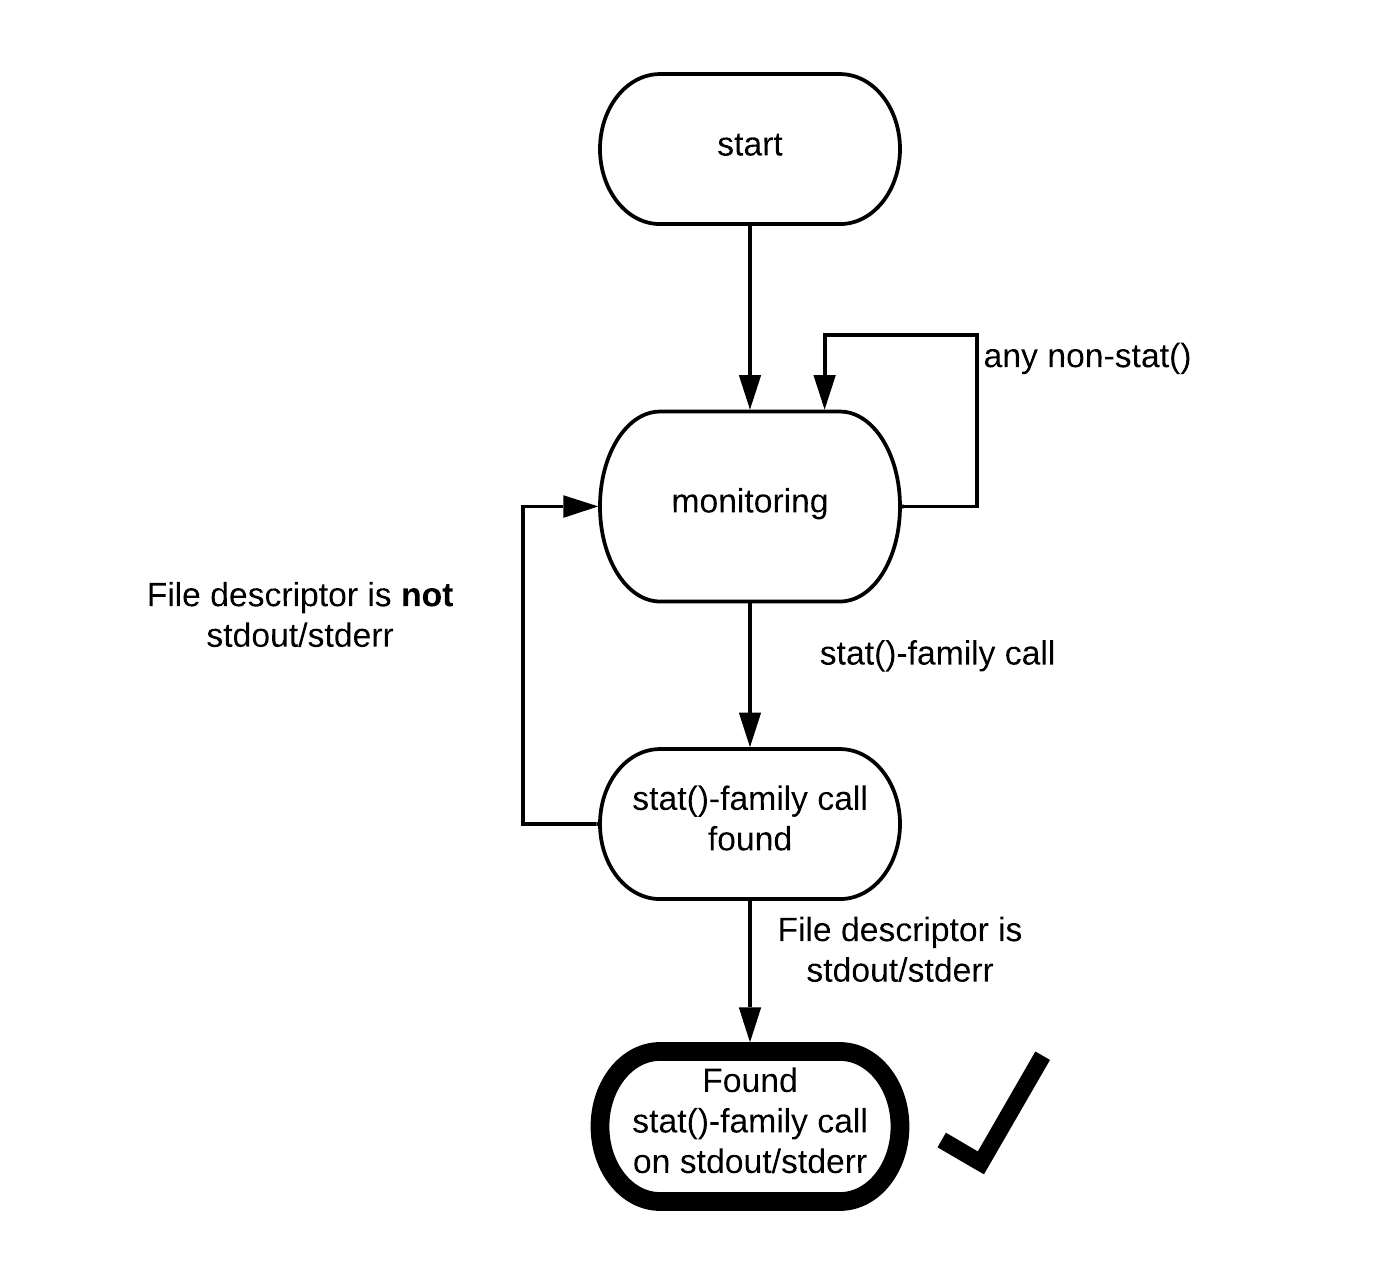
\includegraphics[scale=.6]{images/statidentify}}
  \caption{A mutator simulating the combinations of character devices and
  regular files curl handles must identify a call from the {\tt stat} family
  operating on the {\tt stderr} or {\tt stdout} file descriptor.  It
  can then modify the returned structure to simulate a given combination.}
  \label{figure:statidentify}
\end{figure}

As a real-world example
of building checkers and mutators
consider the measures {\tt curl} takes
to ensure it properly outputs the data it retrieves from a url.
By default,
curl outputs the contents of the requested url to the terminal.
In cases where {\tt stdout}
refers to a file, curl instead outputs a progress bar to the terminal by
writing to {\tt stderr}.  In a third case where both {\tt stdout} and {\tt
stderr} are redirected to files curl omits this progress bar entirely, as it could
interfere with the data being retrieved from the url should curl's
user specify a configuration where both {\tt stdout} and {\tt stderr} are
redirected to the file.

{\tt Curl} determines the configuration of {\tt stdout} and {\tt stderr}
by using a system call from the
{\tt stat} family.  Specifically, calls from this family return a structure that
contains, among other information, a bitmap that denotes the Linux file type of
the file being examined.  Evaluating this bitmap allows an application to
determine whether a file descriptor points to a data file
(a regular file) or the terminal (a character device).  Well-behaved applications should make these checks and alter
their output accordingly.

Figure~\ref{figure:curlflow} illustrates the combinations of regular files and character devices
that curl looks out for.  SEA allows for the construction of a mutator and
a checker that can test other applications against the same set of
combinations.  Such a mutator would identify {\tt stat}-family system calls
performed upon the {\tt stdout} and {\tt stderr} file descriptors and alter
their results to simulate the desired combination.
See figure~\ref{figure:statidentify}
for a diagram of a potential underlying automaton for this mutator.
Some indication of the
correctness of an application's response to the simulation could be gained by a
checker that simply looks for the application to change its behavior in
unexpected cases (i.e. the default checker).


\subsection{CrashSimulator: A Concrete SEA Implementation}
\label{SUBSEC:ApproachCrashSim}

In order to correctly implement SEA, CrashSimulator
must provide a framework
by which the checkers and mutators
constructed by its users can be used to
test an application using the anomalies they represent.
Building this capability
required making a few key design decisions. The first, as mentioned in
Section 2, was choosing to operate at the system call level, rather than
manipulating calls to library functions, memory accesses, or other points
where we could influence an application's interactions.
This allowed CrashSimulator
to test applications written in any
language that can execute Linux system
calls -- an important advantage as our
goal is a tool that can test many
applications without per application
effort.
Working with system calls is also a good fit
for simulating the file system,
network, and operating system anomalies in which we were interested.
An application normally queries these entities using system calls
so we simply had to return modified responses in order to simulate an
anomaly.
Finally, robust tooling in the Linux kernel made the
interception and modification of system call results and side effects a
fairly simple process,  and the well-defined semantics of Linux
system calls streamlined implementation.


In order to take advantage of our ability to simulate anomalies using
system calls, we needed to ensure that an application would reliably make
the same set of
system calls, and reach the same simulation opportunities,
with every execution.
To this end,
we employed a modified
{\tt rr} debugger~\cite{rrwebsite} to record and replay applications. Our
first modification permitted a {\tt strace}-style system call recording
to be output alongside {\tt rr's} normal recording format,
creating a complete log of an application’s system call activity.
We chose to make this
modification because, while {\tt rr}'s recording contains the system call
information we need, it is stored in an opaque format that changes
frequently between versions.  Storing a copy of this information as a {\tt
strace} recording bypasses this shortcoming and offers the advantage of
being human readable.

Our second modification parallelized our testing
by allowing {\tt rr} to generate copies of a running application when
it reaches our target simulation opportunities.
We refer to this new technique as {\it process set cloning}
and illustrate it
in Figure~\ref{figure:architecture}.
The {\tt rr}
debugger manages, and can copy, the full set of processes underlying an
application so that users can test debugging hypotheses without damaging
the original.  We extended this capability by liberating process
set copies from {\tt rr}.  This means that given application $Y$ consisting
of processes $a$, $b$, and $c$ (written as $Y(a, b, c)$), we can generate
cloned sets $Y_1(a_1, b_1, c_1)$, $Y_2(a_2, b_2, c_2)$ ... $Y_n(a_n, b_b,
c_n)$.  $Y_1$, $Y_2$ ... $Y_n$ can then be used to test different
scenarios.  These clones can be run in parallel because they do not
actually execute system calls or modify the operating system state.
Instead, they are simulated as described below.
Additionally,
they allow the original $Y$ to continue its execution unhindered.

Once generated, the cloned process sets are used
for testing by the CrashSimulator process supervisor.
This supervisor is responsible for attaching to a process set
via {\tt ptrace} and
servicing any system calls it makes.
The data required to service these calls
comes from the  {\tt strace} log
generated by {\tt rr}.
Just before it takes over service of system calls,
the process supervisor invokes the intended anomaly's mutator
on the log in order to alter it to include the responses
necessary to simulate an anomaly.
Once these alterations are in place,
the supervisor is able to impose an anomaly
on the application by returning the now-modified responses from the log.

During this process,
a corresponding checker
monitors the application's behavior,
allowing it to report on the correctness of the response.
For example, testing could proceed in the following way.
At a given simulation opportunity, when executing application $Y$,
cloned sets $Y_1$ and $Y_2$ are generated and
used to test two scenarios where a file access could fail:
\begin{enumerate}
    \item{For $Y_1$, access to the file is denied due to a permissions issue}
    \item{For $Y_2$, access fails because of an I/O error}
\end{enumerate}
The simulations for both $Y_1$ and $Y_2$ are handled asynchronously and
the results are recorded.
This approach allows many tests to be run independently of one another,
which lends a
high degree of speed and
parallelism to the testing process.
At the same time, the original $Y$ execution continues unhindered to the
next simulation opportunity where this process repeats.
Keeping the original execution intact,
as opposed to destroying it by introducing an error state,
avoids the penalty
of having to restart a new execution for each test.

\begin{figure}[t]
  \center{}
  \fbox{\includegraphics[scale=.37]{images/architecture}}
  \caption{Diagram illustrating CrashSimulator's architecture.  During the
    course of a single rr execution, clone process sets are generated at
    specific rr events.  A CrashSimulator process supervisor attaches to
    these process sets and uses a strace-style system call listing to feed
    subsequent system call activity and inject unusual environmental
    conditions.}
  \label{figure:architecture}
\end{figure}

The prototype was built on rr version 5.2.0 running on a 32-bit Linux kernel
distributed with Ubuntu 16.04 LTS.  The modifications to rr described above
were carried out in C++, and the CrashSimulator
supervisor was implemented in 6260 lines of Python 2.7 code with a 2125
line C extension that allows it to interact with processes using the Ptrace
API.
This version of CrashSimulator is available at:
https://github.com/pkmoore/rrapper.

\input{implementation}
\section{Evaluation}
\label{SEC:evaluation}

CrashSimulator was designed
as a way to reduce the considerable effort
required of developers to test an application
against the environments it will encounter once deployed.
Therefore,
we needed to demonstrate its effectiveness in ``the wild.''
To this end,
we carried out two rounds of
evaluation for CrashSimulator.
We started by exposing
a series of real-world applications
to a library of collected anomalies in a laboratory environment.
These tests,
conducted by the research team,
were followed by a user study
in which undergraduate and graduate computer science students
got a chance to use CrashSimulator
to identify new environmental bugs
in tests on applications of their choosing.
We used the results from both these efforts
to answer the following questions:

\begin{enumerate}

\item{Is CrashSimulator able to identify bugs in real world applications?
    (Subsection~\ref{sec-env-bugs})}

\item{What sorts of errors does CrashSimulator make?
    (Subsection~\ref{sec-sorts-errors})}

\item{Can CrashSimulator
      execute tests efficiently? (Subsection~\ref{sec-perf})}

\end{enumerate}

\subsection{Is CrashSimulator able to identify bugs in real world
applications?}
\label{sec-env-bugs}

The most crucial question to ask about the SEA technique and the tool we
implemented is:
can we use them to identify bugs
caused by different types of problematic environmental features?
To perform this evaluation we needed both a set of applications to test
and a set of anomalies against which to test them.
In order to show that CrashSimulator
can find bugs in even the most widely deployed
and well tested applications,
we chose our test candidates
from among those deemed ``popular''
by Debian's Popularity Contest~\cite{DebPopCon},
or those used
by many Linux distributions,
such as the ones provided
by the GNU coreutils project.

To prove the breadth of CrashSimulator's capabilities we needed
to test applications
using a diverse set of exemplar anomalies.
We already established
that
unusual filesystem and network situations can cause an application to fail.
So we identified a number of candidate anomalies
by examining public bug trackers,
the source code of major portable applications, and the capabilities of
bug finder tools like NetCheck~\cite{Zhuang_NSDI_2014}
and CheckAPI~\cite{rasley2015detecting}.
From these candidates we
chose to three test scenarios: a simple filesystem anomaly that relies on the null
mutator;
a more complex filesystem anomaly that simulates
the presence of unusual file types;
and a network anomaly that requires
checking and mutating many values across a variety of system calls.
Our experiences testing applications with these anomalies are detailed below.

\subsubsection{The simplest case - A Filesystem Bug Found With the Null Mutator}
\label{sec-move-bugs}
In our first test we decided to evaluate the tool in its simplest possible
configuration -- employing the {\bf ``null mutator.''}
This mutator takes no action and simulates no anomalous conditions.
It simply allows checkers to evaluate an application's behavior
as it carries out a potentially-buggy operation.
We decided to look at how applications
move files around on the filesystem.
Though, in many cases, this operation can be handled
atomically by the operating system
through the {\tt rename()} system call,
in situations where
the source file and destination file are on different storage devices,
the application must perform the operation in a more complex way.
This is a process
that even well-tested applications
frequently get wrong~\cite{PHPRenameBug,PythonShutilBug,NodejsCopyBug}.

{\bf Method.}
CrashSimulator was configured
to test each of the applications listed in Table~\ref{table:crossdevice}
to see which might fail to correctly move a file from one disk to another.
The tests were completed using just the Null Mutator and a set of
checkers that model the correct steps involved in moving a file from one
storage device to another.
After examining several libraries and applications,
we found that
{\tt mv} seemed to handle cases that other tools failed to consider.
Therefore, we
used its behavior as a template to create a set of checkers
that evaluate whether or not
the application correctly performs the following
steps.

\preston{I put these more detailed descriptions back}
{\it Source Replaced.} An application should make an effort
to ensure that the file being copied
is not replaced between the time it is initially examined
and the time it is opened for copying.
Otherwise,
it could have been replaced by a file of a different type,
such as a character device.
To test whether applications are robust
to anomalies involving source file replacement,
we developed a checker that monitors whether a series of safety checks
are performed.
If these checks are not performed it
means the application will proceed with its operations,
leaving open the possibility of file corruption~\cite{PythonShutilBug}.

{\it Preserve Xattrs} Extended file attributes
are used by modern operating systems
to store descriptive information
that the strictly defined and limited structure
of normal filesystem fields cannot hold.
For example,
an operating system can use extended file attributes
to record whether or not a file was downloaded from the Internet.
This is important security information
that is used to warn users
if they are about to open a potentially unsafe file.
Apple's Gatekeeper relies on extended file attributes
to prevent the execution of applications downloaded from
untrusted developers without explicit user action~\cite{AppleCodeSigning}.
When copying a file,
an application should retrieve extended file attributes from the source
file and, later, apply them to the destination file.
In this case, CrashSimulator used a checker
that watches for the application to make system calls
that read the extended file attributes from the source file (i.e. {\tt
  getxattr()}, {\tt lgetxattr()}, or {\tt fgetxattr()}) followed by system calls
that re-apply the attributes to the destination file (i.e. {\tt setxattr()},
{\tt lsetxattr()}, or {\tt fsetxattr()}).

{\it Preserve Timestamps} Incorrect timestamps can impede applications like
in {\tt make}, archival programs, and similar
software~\cite{NautilusTimestamps, SudoTimestamp}.
As a result, it is important to ensure
that time related metadata --
such as creation, modification, and access times
are preserved when copying a file.
To evaluate failures on this front,
we used a checker that determines
whether the application applies
the appropriate timestamps to the destination file
by monitoring for system calls from the {\tt stat()}
and {\tt utime()} families used to retrieve and apply timestamps.

{\it Copying Devices} It is also important to check if a move
would attempt to copy a special
device file, such as a named pipe, across disks.
Files of this variety must be moved
by creating a new device of the same type at the destination,
instead of exhaustively reading and writing its contents.
In our experience, applications that fail to perform this check
can end up completely filling a disks, exhausting available memory,
or blocking forever, which can cause the system to become unresponsive.

% Temporarily commented out in favor of more detailed versions that were
% cut for length

% \begin{itemize}
%     \item{{\it Confirm Source Not Replaced During Copy.} An application
%         should make an effort to ensure that the file being copied is not replaced between the time it is initially examined and when it is opened for copying.
% If these checks are not performed, it
% means the application will proceed with its operations,
%         making file corruption~\cite{PythonShutilBug}} possible.
% 
%     \item{{\it Preserve Extended File Attributes.}
% When copying a file,
% an application should retrieve extended file attributes from the source
% file and, later, apply them to the destination file.  Failure to do so can lead to security problems~\cite{AppleCodeSigning}.}
% 
%     \item{{\it Preserve Timestamps.}  It is important to ensure
% that time related metadata --
% such as creation, modification, and access times  --
% are preserved when copying a file, as
% incorrect timestamps can impede applications like {\tt make},
%         archival programs, and similar software~\cite{NautilusTimestamps,
%         SudoTimestamp}.}
% 
%     \item{{\it Copy Devices Correctly.}
% Files of this variety must be moved
% by creating a new device of the same type at the destination,
% instead of exhaustively reading and writing its contents.
% In our experience, applications that fail to perform this check
% can end up completely filling disks, exhausting available memory,
%         or blocking forever, which can cause the system to become unresponsive.}
% 
% \end{itemize}

 \begin{table}[t]
    \scriptsize{}
    \begin{tabular}{l p{1cm} p{1cm} p{1.2cm} p{1cm}}
    \toprule{}
        Application     & Source Replaced & Preserve Xattrs & Preserve Timestamps & Copying Devices\\
\hline
        {\tt mv}              & Correct             & Correct         & Correct             & Correct\\
        {\tt mmv}             & Correct             & {\bf Sec. Flaw} & {\bf Time Loss} & Correct\\
        {\tt install}         & Correct             & {\bf Sec. Flaw} & {\bf Time Loss} & {\bf Fill Disk} \\
        {\tt perl File::Copy} & Correct             & {\bf Sec. Flaw} & {\bf Time Loss} & {\bf Fill Disk} \\
        {\tt shutils}         & {\bf Corrupt}	& {\bf Sec. Flaw} 	& Correct             & Correct\\
        {\tt rust}             & Correct             & {\bf Sec. Flaw} & {\bf Time Loss} & {\bf Fill Disk} \\
        {\tt boost::copyfile} & {\bf Corrupt}	      & {\bf Sec. Flaw} & {\bf Time Loss} & {\bf Fill Disk} \\
    \bottomrule{}
    \end{tabular}
    \caption{Applications and libraries analyzed to determine whether or not
      they are able to correctly move a file from one device to another.
Incorrect entries are either missing the needed check to ensure correct
     behavior or their implementation of the behavior was ineffective.}
    \label{table:crossdevice}
\end{table}

{\bf Findings.}
CrashSimulator was able to identify whether an array of popular programs,
including the standard libraries for the programming languages Python,
Perl,
and Rust,
can correctly perform complex
operations in anomalous situations.
As can be seen from the results in Table~\ref{table:crossdevice}, each of the
applications tested failed to perform one or more of the steps required to
successfully complete a cross-device move.  This is an unfortunate situation
because a failure to perform any one of these steps can result in negative
outcomes for the system as a whole.  There was one case where our
checkers made a false positive report which prompted efforts to improve it.
This is discussed further in
Section~\ref{sec-sorts-errors}.
Taken as a whole, our results demonstrate that even well-tested applications
can miss one or more of the steps in a complicated operation.

\subsubsection{A More Complex Case - The Unexpected File Types Mutator}
\label{sec-file-type-bugs}

If a more complex mutator is to be employed, then
CrashSimulator will simulate anomalies as an application is executed.
This simulation introduces problematic scenarios
so an application's response
can be evaluated.
For an effective test of the
tool's capabilities to find bugs created in this process,
we needed to pick an anomaly
that would arise during a common situation,
such as when a Linux application retrieves
and processes data from a file.
Linux supports
several special file types,
including
directories,
symbolic links,
character devices,
block devices,
sockets, and
First-In-First-Out (FIFO) pipes.
These special files
use the same system calls
as regular files
(such as {\tt read()} and {\tt write()}),
but they behave in very different ways.
For example,
{\tt /dev/urandom} is a character device
that produces an infinite amount
of pseudo-random data
when read.
If {\tt /dev/urandom} is provided to an application
that relies on exhaustively reading the full
contents of a file before processing, it
will fill memory or disk space, and could
crash the system~\cite{YumAptEndless}.
Correct execution in these situations
requires that applications
examine the files, so they do not
interact inappropriately with a given file type.

{\bf Method.}
Identifying these bugs involves changing an application's
execution to induce its response to an unexpected file type. For
example, the {\tt sed} application, which modifies the contents of a text
file according to a provided command string, could instead be provided a symbolic
link, a directory, or a character device.  CrashSimulator
tests these alternatives by identifying the calls to {\tt stat()}, {\tt fstat()},
or {\tt lstat()} that an application makes to examine the file, and
changing the results to simulate
one of the special file types.  If the application responds to
this injected information, then the special
file might be handled correctly.  On the other hand, if there is no
alteration in the behavior of the application, the condition is not
being handled correctly.

For each application,
CrashSimulator was configured to simulate all of the non-standard file
types.
The values inserted into results of the application's {\tt stat()}-like
system calls are listed
in Table~\ref{table:unexpectedtypes}.
A value of ``--'' indicates
that this is the file type the application was expecting,
as it matches what was provided when the application was initially recorded.
A result of ``\tickmark'' indicates that the application
identified it was being provided with an unexpected file type and its
execution differs, a signal that it was potentially handling the
file type correctly.
A result of ``X'' indicates
that the execution never diverged from the trace being replayed,
and thus failed to recognize the presence of an unusual file type.

{\bf Findings.}
The data in Table~\ref{table:unexpectedtypes} show that of the 84 cases we
tested, CrashSimulator identified 46 bugs,
predicted 25 instances of correct application behavior,
and made 13 errors,
the majority of which were false negatives.
We discuss the causes of these errors
in Section~\ref{sec-sorts-errors}.
The frequency of failed executions in our results
indicates that many
applications assume they will only be used to process
regular files.  When this assumption does not hold, execution results
can be hard to predict.
In many cases a denial of
service condition occurs in the form of the application ``hanging,'' as it
attempts to incorrectly process the file.
This is typically the result of
an application blocking forever as it waits for a {\tt read()}
call to retrieve non-existent data from an empty FIFO,
or an application attempting
to read in and process an
``infinitely large'' file.
This situation is particularly dangerous as
it can eventually
fill all available memory or disk space~\cite{Cappos_CCS_08}.


\begin{table*}[t]
    \scriptsize{}
    \begin{tabular}{l  l  |  l  l  l  l  l  l  l}
    \toprule{}
        Application       & Condition Tested           & Regular File           & Directory               & Character Device        & Block Device           & Named Pipe                 & Symbolic Link             & Socket File \\
                          &                            &  (IFREG)               & (IFDIR)                 & (IFCHR)                 & (IFBLK)                & (IFIFO)                    & (IFLNK)                   & (IFSOCK)\\
\hline
        {\tt Aspell}      & Dictionary File            & --                     & X: \textit{FP}          & \tickmark: \textit{FN}  & X                      & X                          & X                         & X          \\
        {\tt Aspell}      & File being checked         & --                     & X: \textit{FP}          & \tickmark               & X                      & X                          & X                         & X          \\
        {\tt gnu-gpg}     & secring.gpg                & --                     & X                       & X                       & X                      & X                          & X                         & X          \\
        {\tt vim}         & File being opened          & --                     & \tickmark: \textit{FN}  & \tickmark: \textit{FN}  & \tickmark: \textit{FN} & \tickmark: \textit{FN}     & \tickmark: \textit{FN}    & X          \\
        {\tt nano}        & File being opened          & --                     & \tickmark               & \tickmark               & \tickmark              & X: \textit{FP}             & X: \textit{FP}            & X: \textit{FP} \\
        {\tt sed}         & File being edited          & --                     & \tickmark               & X: \textit{FP}          & X                      & X                          & X                         & X          \\
        {\tt wc}          & File being checked         & --                     & \tickmark               & X                       & X                      & X                          & X                         & X          \\
        {\tt du}          & Directory being checked    & \tickmark              & --                      & \tickmark               & \tickmark              & \tickmark                  & \tickmark                 & \tickmark  \\
        {\tt install}     & File being installed       & --                     & \tickmark               & X                       & X                      & X                          & \tickmark                 & X          \\
        {\tt fmt}         & File being formatted       & --                     & X                       & \tickmark               & X                      & X                          & X                         & X          \\
        {\tt od}          & File being dumped          & --                     & \tickmark               & \tickmark               & X                      & X                          & X                         & X          \\
        {\tt ptx}         & File being read            & --                     & \tickmark               & \tickmark               & \tickmark              & \tickmark                  & \tickmark                 & \tickmark: \textit{FN} \\
        {\tt comm}        & Second file being compared & --                     & \tickmark               & \tickmark               & X                      & X                          & X                         & X          \\
        {\tt pr}          & File being read            & --                     & \tickmark               & X                       & X                      & X                          & X                         & X          \\
\hline
        \multicolumn{9}{l}{\scriptsize{\tickmark  $=$ CrashSimulator
        predicts application will recognize anomaly}}\\
        \multicolumn{9}{l}{\scriptsize{X $=$ CrashSimulator predicts
        application will fail to recognize anomaly}}\\
        \multicolumn{9}{l}{\scriptsize{-- $=$ File type expected by the
        application}}\\
    \bottomrule{}
    \end{tabular}
    \caption{Applications tested for their handling of unexpected file types.  A
    result of ``\tickmark'' indicates that the application identified the
    presence of an unusual file and responded in some fashion.  A result of
    ``X'' indicates that the application failed to recognize the presence of
    an unusual file and attempted to process it.  Cases where
    CrashSimulator made an error are noted by FP (False
    Positive) or FN (False Negative)}
    \label{table:unexpectedtypes}
\end{table*}


\begin{table}[t]
    \scriptsize{}
    \scalebox{.82}{
    \begin{tabular}{l  l  l  l  l  l  l  l  l}
    \toprule{}
        Application         & Directory                 & Character Device & Block Device  & Named Pipe \\
                 & (IFDIR)                   & (IFCHR) & (IFBLK) & (FIFO) \\
\hline
        {\tt wc}            & Error: Is a Directory     & hangs       & slowly process file  & Hangs\\
        {\tt install}       & Error: Omitting Directory & Fills disk  & slowly copies file   & Hangs\\
        {\tt fmt}           & No output                 & hangs       & garbage output       & Hangs\\
        {\tt od}            & Error: read error         & hangs       & No output            & Hangs\\
        {\tt ptx}           & Error: Is a Directory     & fills disk  & garbage output       & Hangs\\
        {\tt comm}          & Error: Is a Directory     & hangs       & garbage output       & Hangs\\
        {\tt pr}            & Error: Is a Directory     & hangs       & garbage output       & Hangs\\
\hline
    \bottomrule{}
    \end{tabular}}
    \caption{Responses of a sample of coreutils applications when exposed to
      anomalous conditions.  The character device used was the infinite-length {\tt
        /dev/urandom}.}
    \label{table:applicationresponses}
\end{table}

In order to confirm the accuracy of CrashSimulator's assessment, we manually
exposed the applications listed in Table~\ref{table:unexpectedtypes} to
each of the unusual file types to get an idea of how they would respond.
This allowed us to identify cases where CrashSimulator made errors and
note this information in Table~\ref{table:unexpectedtypes}.  Further,
we include descriptions of a subset of the applications' behaviors in
Table~\ref{table:applicationresponses}.
These tables serve to document the accuracy of the tool's
evaluation of application behavior and illustrate what misbehavior occurs
when applications are actually exposed to problematic scenarios.
%One possibility is that CrashSimulator asserts
%that the application will fail
%and in practice, it does.  We found this when we evaluated
%the response of  {\tt install} receiving a character device
%rather than a regular file. Our test predicted failure and the
%application ended up filling the disk of the machine on which it was run.
%In other cases, CrashSimulator reported that an
%application had detected the anomalous condition and the application managed to
%do so in practice,  as when we evaluated {\tt wc}'s successful response to
%being run on a directory.

\subsubsection{Beyond Filesystem Bugs - Poorly Configured Network Timeouts}
\label{sec-timeout-bugs}

CrashSimulator is not limited
to identifying filesystem-based bugs.
The third anomaly we examined
involves an application's behavior
when it attempts to communicate
over a network with extremely long
(on the order of minutes) response times.
At a low level,
applications retrieve data from a network socket
by waiting for data to be available and then reading it.
However,
this approach needs to be able to handle
a situation where communication
takes too long and should time out.

{\bf Method.}
CrashSimulator can detect
whether an application correctly times out when communications
take too long
by employing the null mutator and a network timeout checker. The latter
can determine if the application makes any effort
to configure its network communications with a timeout value.
This is done by examining the presence or absence of {\tt setsockopt()}, {\tt poll()}
and {\tt select()} calls, as well as the timeout values that may
have been passed to them. Applications that do not set the timeout are
subject to the operating system-defined protocol timeout value.
CrashSimulator is able to take this analysis a step further by employing a Long Network Response Time mutator
that manipulates
the results of all time-returning calls,
simulating an execution where close to the maximum timeout value occurs,
without actually spending any time waiting.

An application's failure
to time out responsibly
is not just an inconvenience. Attackers can take advantage of this flaw
to consume resources and potentially cause a denial of service situation.
This failure was exploited by the slowloris~\cite{Slowloris} tool
to enhance the ability
of a small number of computers to prevent access
to vulnerable web servers
by opening and maintaining connections
for extremely long periods of time.
As these servers could only handle a set number of connections
due to resource constraints,
legitimate traffic was easily crowded out by the attackers.
Additionally, similar attacks can be used to
indefinitely delay security updates to
clients, leaving them vulnerable to compromise~\cite{Cappos_TR_08}.
We used CrashSimulator to determine which applications and
libraries from a selection based on Debian's ratings~\cite{DebPopCon}
could be vulnerable to this sort of attack.

\begin{table}[t]
  \scriptsize{}
  \begin{tabular}{l | l}
    \toprule{}
    {\bf Application}              & {\bf Analysis Result}\\
    {\tt wget}                     & Overly long timeout supplied to {\tt select()} \\
    {\tt ftp}                      & No {\tt poll()} or {\tt select()}, no timeout set \\
    {\tt telnet}                   & {\tt select()} specifies no timeout \\
    {\tt urllib http}              & No {\tt poll()} or {\tt select()}, no timeout set \\
    {\tt urllib ftp}               & No {\tt poll()} or {\tt select()}, no timeout set \\
    {\tt ftplib}                   & No {\tt poll()} or {\tt select()}, no timeout set \\
    {\tt httplib}                  & No {\tt poll()} or {\tt select()}, no timeout set \\
    {\tt requests}                 & No {\tt poll()} or {\tt select()}, no timeout set \\
    {\tt urllib3}                  & No {\tt poll()} or {\tt select()}, no timeout set \\
    {\tt python-websocket-client}  & No {\tt poll()} or {\tt select()}, no timeout set \\
    \bottomrule{}
  \end{tabular}
  \caption{Applications tested for their handling of extremely slow response
    times from the host with which they are communicating }
  \label{table:slowloris}
\end{table}


{\bf Findings.}
As Table~\ref{table:slowloris} shows, all of these
applications were vulnerable to this anomaly,
and in some cases,
timeouts took hours to resolve.
What's more, in the vast majority of
cases, the problem occurs because the application makes no effort to
specify a timeout value.  This means an attacker can transmit one byte of
data per timeout period (per Linux's value of 19 minutes for TCP sockets),
allowing them to keep the application alive instead of quitting.

\subsubsection{Bugs Found By Participants}
Because the above tests were carried out by CrashSimulator's developers,
who necessarily have a high degree of expertise in its operation,
we felt it prudent to ensure the tool was useful
to outside developers as well.
To investigate this angle,
we conducted a user study
with 12 undergraduate and graduate students with varying backgrounds.
Study participants found a total of 11 bugs using CrashSimulator.
Of these bugs, nine were found using the ``Unusual Filetype'' mutator.
Five of these bugs have since been reported to the appropriate maintainers,
and three of these reports included patches
that correct the bug
built by the reporting student.

These results are important
because they confirm
users, other than the original development team,
can use the tool to find bugs in real world applications.
Participants commented that narrowing the source of a bug
down to a particular sequence of system calls
was helpful in identifying the area of
code responsible for the bug -- a feature
that decreased the time required to produce a fix.
Though observation of study participants
showed that familiarity with operating systems concepts
made it easier to work with CrashSimulator,
those without this background were still able to identify bugs using the
built in anomalies.

On a less positive note,
the study did reveal
some shortcomings
of the tool.
First,
it became clear that the tool
does not have a clear mechanism
for determining
which application behaviors constitute a ``bug.''
For example, an application's developer
may have intended that an application processing an ``infinitely long'' file should run continuously
until killed by an outside command.
Therefore, that behavior should not be classified as a bug.
Second,
it demonstrated that
simply reporting that an application did or did not change its behavior
in the presence of an anomaly may not provide sufficient data to identify a bug. The results indicating the presence of a bug must be clear to the user.
Both of these issues are being corrected
by improving the tool's outputs.
By more clearly describing
the nature of a given result,
users can have a better idea
if,
and why,
they should be concerned.


\subsection{What Sorts of Errors does CrashSimulator Make?}
\label{sec-sorts-errors}

Like other testing tools, CrashSimulator occasionally makes mistakes.
Any such mistakes can
undermine a developer's confidence in a tool, and thus one of our goals is
to minimize them.   In this section, we discuss
situations where CrashSimulator made either false positive or false
negative reports.  A false positive report means the tool reports
a failure when the application actually handles an anomaly correctly.
On the opposite side, false negative reports happen when the tool indicates an application handles
an anomaly when, in reality, it does not.

\textbf{False Positives.}
The primary source of false positives in CrashSimulator is an application
responding to an anomaly with a different sequence of system calls
than was expected by the checker.
Once identified, CrashSimulator's approach allows these
situations to be easily corrected.
This is similar to a situation
where an application's test suite
has a test with an over-constrained ``oracle''
(e.g. an oracle that ensures a returned value is $>0$ when, in reality,
$0$ is acceptable).

We encountered this situation when testing applications that used
GNOME's {\tt glib} file handling functions.  When an
application makes use of these facilities to move a file across storage
devices, the library itself correctly performs a
file move operation.  When we used CrashSimulator with
checkers that expected a call to {\tt read()} and {\tt write()}
for a cross-device move, we got reports stating that the
application {\em did not} perform the system calls necessary to
correctly move a file.
By manually
examining a system call trace, we found that, while {\tt glib} correctly
performs the requested move operation,
it does so using alternative system call
sequences.  Rather than using a sequence of {\tt read()} and {\tt write()}
calls, as our checker expected, {\tt glib} creates a pipe and uses the {\tt
splice()} system call to copy the contents out of the source file, through
the pipe, and into the destination file.

Fortunately, as soon as issues like this are discovered,
CrashSimulator's checkers can be modified to include the alternative
sequence.
Given the above example about moving
files, consider the mapping from high level ``operation'' to the set of
system calls that can implement it in Table~\ref{table:stepsandcalls}.
Each of the steps in the operation map to a small number of system calls.
In
situations where two system call sequences can correctly implement the same
operation, CrashSimulator simply runs two checkers in parallel
and accepts the execution if either detects the expected sequence.

\begin{table}[t]
    \scriptsize{}
    \begin{tabular}{l | l }
    \toprule{}
      {\bf Operation}                                               & {\bf Potential System calls}\\
      Examine source file                                     & stat64(), lstat64(), fstat64()\\
      Examine destination file                                & stat64(), lstat64(), fstat64()\\
      Open source file                                        & open()\\
      Read contents of source file                            & read(), splice() with a pipe\\
      List source file's & \\ ~~~~~extended file attributes             & listxattr(), llistxattr(), flistxattr()\\
      %Read contents of source file's extended file attributes & getxattr(), lgetxattr(), fgetxattr()\\
      Read contents of source file's                    & \\
      ~~~~~~~extended file attributes & getxattr(), lgetxattr(), fgetxattr() \\
      Open destination file                                   & open(), optionally unlink() the file first\\
      Write contents to destination file                      & write(), splice() with a pipe\\
      Apply extended file attributes to & \\ ~~~~~destination file      & setxattr(), lsetxattr(), fsetxattr()\\
      Apply proper timestamps to & \\ ~~~~~destination file             & utimens(), futimens()\\
      Apply proper permissions & \\ ~~~~~to destination file            & chmod(), open() with a modeline specified\\
      Close the source file                                   & close()\\
      Close the destination file                              & close()\\
    \bottomrule{}
    \end{tabular}
    \caption{Each step of a successful cross-disk file move operation mapped to
      the system call or calls that can implement it}
    \label{table:stepsandcalls}
\end{table}

%A second source of false positives is a test being configured such that not
%enough of the application's execution is included in the test.
%One implementation detail of CrashSimulator is that,
%by default,
%its tests evaluate an application's behavior
%within a defined (but configurable) number of system calls.
%We found in some cases
%that an application's error handling or recovery code
%may take place outside of this span of execution.
%False positives
%of this sort
%are easily corrected
%by expanding the length of execution
%covered by the test.
%The low number of occurrences of this
%type of false positive gives us confidence that the default configuration
%is satisfactory in the majority of cases.

\textbf{False Negatives.}
False negatives are a fact of life in testing
because of missing test cases or under-constrained checks
of result correctness.
CrashSimulator occasionally registers  false negative reports
when an application changes its behavior,
but does not handle an anomaly correctly.
In our evaluation we encountered ten such reports, four
occurring with one application, {\tt wc}.
Because these reports were generated when using the default checker,
they can be addressed by
using a more elaborate checker that
performs a detailed analysis
of the application's post-simulation behavior.
Such a checker would compare this behavior to a model of
a correct response to that anomaly.
Creating this checker requires
that a user know
what a ``correct response''
looks like.
This ``known good'' behavior can be found
by looking at standards and documentation
that describe best practices for handling an anomaly
in a given environment,
or by examining how applications that correctly
deal with the anomaly do so.
Consider the case where a {\tt close()} system call fails.
Retrying the call may not be the correct action,
depending upon the environment in question.
SEA can be used to determine if an application
has handled the failure correctly
by examining post-simulation communications in detail,
and taking into account the correctness of retrying the call.

\subsection{Can CrashSimulator execute tests efficiently?}
\label{sec-perf}

One key attribute of successful testing tools is that they are able to
complete their tests in a timely manner.  If a tool takes too long,
users will be less likely to run it.
To address this concern,
we evaluated CrashSimulator's performance
in order to determine whether or not it was able to complete its
test executions in an acceptable time frame.

{\bf Method.}
To answer the question of performance, we examined the completion
times for executions of the specified application in both
native conditions, and under CrashSimulator configured to test using the ``Unusual File
Types'' anomaly discussed earlier.
Table~\ref{table:performance} shows these results.

%    \begin{figure}[t]
%        \center{}
%        \fbox{\includegraphics[scale=.75]{images/performance.png}}
%        \caption{\emph{This shows the run time difference between the
%native program and CrashSimulator in seconds.  Each dot indicates an
%        execution.  The X axis shows time values for native executions, and
%        executions under CrashSimulator with 0, 5, 10, and 100 tests
%        performed respectively.
%}}
%         \label{figure:performance}
%
%    \end{figure}

 \begin{table}[t]
    \scriptsize{}
    \begin{tabular}{l p{1cm} p{1cm} p{1.2cm} p{1cm}}
    \toprule{}
        Application     & Native Execution Time & Initial Recording Time & CrashSimulator Replay Time & rr Replay Time  \\
\hline
        {\tt wc}        & 0m0.007s              & 0m0.473s               & 0m0.668s                   & 0m0.112s        \\
        {\tt fmt}       & 0m0.007s              & 0m0.321s               & 0m0.707s                   & 0m0.111s        \\
        {\tt od}        & 0m0.036s              & 0m0.317s               & 0m0.689s                   & 0m0.101s        \\
        {\tt ptx}       & 0m0.008s              & 0m0.352s               & 0m0.769s                   & 0m0.087s        \\
        {\tt comm}      & 0m0.132s              & 0m0.371s               & 0m0.776s                   & 0m0.141s        \\
        {\tt pr}        & 0m0.135s              & 0m0.888s               & 0m1.017s                   & 0m0.141s        \\
    \bottomrule{}
    \end{tabular}
    \caption{This table contains the times required to execute several coreutils applications under different conditions.
             Native execution time is the time required to execute the application from the command line while
             CrashSimulator Replay time is the time required to execute it with the tool, using the null mutator with no checker configured.
             Initial recording time is the time required to create an initial recording with CrashSimulator.  rr replay time is the
             time required to replay an application using rr without CrashSimulator and is included to demonstrate the additional
             overhead added by CrashSimulator's other components.}
    \label{table:performance}
\end{table}


{\bf Findings.}
Overall, the performance running an application
under CrashSimulator is around
two orders of magnitude slower
than the original program executed without it.
As can be seen in Table~\ref{table:performance}, around 20\%
of this slow down is related to the additional overhead of {\tt rr}'s replay.
An additional portion is caused by the need to spin up Python's interpreter
before testing can begin.
In most cases
this slowdown is somewhat mitigated by CrashSimulator's ability to process
tests asynchronously. In other situations, it will be more efficient than
running the program natively, as {\tt rr's} replay does not require
actual execution of most system calls.  This means that CrashSimulator
avoids the system call overheads, such as I/O.
Even without these improvements, however, CrashSimulator's performance
cost is more
than manageable when the value it provides is taken into account.  The
cumulative runtime required to execute the tests required to produce the
results listed in Table~\ref{table:unexpectedtypes} is around 90 seconds.

\section{Testing Usability and Effectiveness on a Wider Audience}

While the results documented in the previous section suggest that CrashSimulator
is effective at finding environmental bugs, we acknowledge that the evaluation
was conducted by developers with a high degree of expertise in its operation,
namely the people who developed it.  We felt it would be prudent to ensure it
would be equally effective when employed by outside developers.
To investigate this angle,
we conducted a user study
with 12 undergraduate and graduate students from with varying experience levels.
This study took place over the course of 6 \preston{check this number} sessions
of an Application Security class attended by both undergraduate and graduate
students.  Each class began with 20
minutes of of instruction on aspects of using the tool
and the remaining 70 minutes were used as work time during which students could
use CrashSimulator to find bugs in applications and construct patches to fix
them.  In addition to this time, students were encouraged to spend time outside
of class furthering their efforts.  They were asked to record their progress
using a provided work log template.


Our goal for this user study was two-fold.  First and foremost,
we wanted to see if the students wereable to use it to find bugs,
even with only limited instruction and experience witht he tool.
We discuss these results in~\ref{subsec:bugs-by-participants}.
Second, we wanted the students to help us identify usability issues
or flaws within the tool itself.  We summarize what the students found
in~\ref{subsec:crashsim-patches}.  Finally, we share our observations
of how students interacted with the tool an what shortcomings
it revealed in~\ref{subsec:tool-shortcomings}.

\subsection{Bugs Found by Participants}
\label{subsec:bugs-by-participants}
Study participants using CrashSimulator found a total of 11 bugs.
Of these bugs, nine were found using the ``Unusual Filetype'' mutator.
Five of these bugs have since been reported to the appropriate maintainers,
and three of these reports included patches
that correct the bug
built by the reporting student.

These results are important
because they confirm
users other than the original development team,
can use the tool to find bugs in real world applications.
Participants commented that narrowing the source of a bug
down to a particular sequence of system calls
was helpful in identifying the area of
code responsible for the bug -- a feature
that decreased the time required to produce a fix.
Though observation of study participants
showed that familiarity with operating systems concepts
made it easier to work with CrashSimulator,
those without this background were still able to identify bugs using the
built in anomalies.

\subsection{Tool Limitations Identified by Participants}
\label{subsec:crashsim-patches}

As we will explain in more detail in our Future Work section,
we believe building a community around CrahSimulator is essential to its
continued development and adpotion.  Our user study proved the correctness
of this assumption.
Students submitted five patches over the
course of the study period to the tool's code.
Three of these patches fixed or enhanced areas of
the tool's documentation, while the remaining two patches fixed issues with the
Dockerfile used to build a container with CrashSimulator installed.

The students also submitted 33 reports pertaining to bugs in CrashSimulator.
Of these, 16 specifically requested support for a new system call that
CrashSimulator had not handled before.  The remaining 17 reported bugs in
existing system call handlers or test orchestration code.
On the one hand this is encouraging.  The necessity of adding
support for new system calls
indicates that the students were
using CrashSimulator against a wide variety of new applications.
On the other hand, the number of bug reports not related to system call support
indicates there is still work to be done on the tool.
It is our goal that progress on both of these fronts will be driven by
CrashSimulator's community.

\subsection{Tool Shortcomings Identified by Observation of Participants}
\label{subsec:tool-shortcomings}
Observations of the students as they used the tool were also revealing.
First,
it became clear that the tool
does not have a clear mechanism
for determining
which application behaviors constitute a ``bug.''
For example, an application's developer
may have intended that an application processing an ``infinitely long'' file should run continuously
until killed by an outside command.
Therefore, that behavior should not be classified as a bug.
Second,
it demonstrated that
simply reporting that an application did or did not change its behavior
in the presence of an anomaly may not provide sufficient data to identify a bug. The results indicating the presence of a bug must be clear to the user.
Both of these issues are being corrected
by improving the tool's outputs.
By more clearly describing
the nature of a given result,
users can have a better idea
if,
and why,
they should be concerned.

{\textbf To Conclude}, our user study has revealed both strengths and weakness
with CrashSimulator.  Our future work section~\ref{sec:future-work}
discusses our plans to improve
these weak areas and capitalize on the tool's strengths.

\input{related-work}
\section{Future Work}
\label{sec:future-work}

The ultimate goal of our future work on SEA and CrashSimulator is to build
a large, self-sustaining community of users around this technique and tool.
%To achieve this we have a
%plan that focuses on both improving the tool and making specific
%community building efforts.  In this section we detail what specifically
%needs to be done to accomplish both parts of this plan.
%
%
%In addition to new feature additions, CrashSimulator requires some updates to
%replace soon-to-be unsupported components.  This includes migration from
%Python 2 to Python 3.  We have migrated several widely used projects that have
%successfully migrated from Python 2 to 3, including TUF~\cite{TUFwebpage}.
%While this will take time, it does not pose substantial risk.
%\cappos{Python 2-3 is optional, cut if the space is needed.}
%
%dependency that requires updating is the processor architecture
%that CrashSimulator supports.  Because the tool performs its simulation
%work manipulating the memory and register values that contain the results
%and side effects of system calls, the initial version of the tool was
%constrained to only supporting x86, 32-bit systems in order to development
%time.  At this point, 64-bit systems (typically x86\_64) are the norm and
%many Linux distributions are reducing the effort put into their 32-bit
%flavors.  While it is possible to use CrashSimulator to test applications
%by re-compiling them for 32-bit x86, this reduces two of the tool's
%advantages -- the ``universal'' nature of its tests and its ability to test
%an application without its source code.  In order to avoid a cumbersome
%situation where is users must recompile their applications, CrashSimulator
%will be changed to support applications compiled for x86\_64.
%
%
%
We propose three areas of improvement in this work.  First, we
will work on enhancing the {\bf usability} of CrashSimulator, in both stand-alone
applications and in integrations into common toolchains.
This is needed
to make the tool more accessible to developers with differing levels of
expertise.
Second, we will address {\bf security} issues by creating
mechanisms that can safely execute mutators and checkers from
untrusted sources.
Third, we will build a website that will facilitate sharing mutators and
checkers with the larger {\bf community}.
We describe each of these in more detail below.


%\subsubsection{Tool Improvements and New Features}
%
%To make CrashSimulator more appealing to our target users we propose taking
%the following actions:


%JAC: This won't work.  You lose the meaning of the anomaly in most cases
% when moving to that level of abstraction.
%\subsubsection{Supporting new platforms}
%
%CrashSimulator has been shown to be successful at finding
%environmental bugs in Linux applications. While this is useful,
%there is a great deal of opportunity to find more interesting, impactful
%bugs by examining the environmental differences resulting from applications
%running on completely different operating systems.
%In order to find these
%bugs, CrashSimulator must be improved so that it can run on, and simulate
%anomalies present in, these additional platforms.  Initially we plan to
%support Windows and OS X.
%
%Key to realizing this support is dealing with the fact that each operating
%system provides different system calls.  For example, Linux uses {\tt
%open()} to open files while Windows provides {\tt NtOpenFile()}.  In their
%current form, checkers and mutators describe anomalies and expected
%application behavior in terms of Linux system calls.  Addressing this
%limitation means elevating this description to a higher level and
%implementing a layer to translate this description down to the actual
%system calls a given operating system provides.  Building upon the previous
%example, a higher level description in a mutator may specify an operation
%like ``open file'' which is translated to either {\tt open()} or {\tt
%NtOpenFile()} as is appropriate.
%
%An additional area for exploration is determining whether or not a given
%anomaly is able to be simulated on a given operating system.  If an anomaly
%only appears in the presence of a operating system feature , it would be an
%error to simulate it on operating systems where this feature is not
%present.  Classifying anomalies in terms of where it makes sense to
%simulate them would reduce the number of false positive reports the tool
%could make.


\subsection{Usability: Grouping and Prioritizing Anomalies}

Not every flaw found by CrashSimulator is equivalent.  An issue that only
impacts an obsolete, rarely used file system is much less impactful than
one that makes the most popular file system vulnerable.
Anomalies
can be prioritized by grouping them into sets representing each
environment in which an application is expected to run. The more popular
the environment, the more the developer may want to be aware of the issue.
It may also be the case that developers want to prioritize fixing all
critical issues for one environment over another.  For example, a piece
of software used in the cloud may not need to worry about issues that will only
occur behind the great firewall of China, if no cloud environments are deployed in this location.


%Grouping by environment and letting the developer prioritize and filter
%environments enables much better developer control and increases the useful
%true positive rate of CrashSimulator.
%For example, the corpus of anomalies included with a future version of CrashSimulator
%could be segregated into groups such as those present on Windows 10, those
%present on Ubuntu 18.04 and so on.  Once grouped in this fashion,
%applications could be tested against a chosen group in order to see how it
%would perform on the represented operating system without. In this way,
%CrashSimualtor could offer insights into how an application will perform on
%a given operating system without having to go through of the effort of
%deploying it.
%
%

\subsubsection{Improving Usability via Integration into CI platforms}

As with other tools, CrashSimulator can only be effective if it is used.
Modern development processes include a continuous integration system,
such as TravisCI
and CircleCI, that run tests automatically.
CI systems are popular because they
ensure that applications are continually and thoroughly tested as new code
contributions are submitted.  Given CrashSimulator's ability to test
applications regardless of how they were constructed,
the tool is a perfect fit for
automatically testing numerous applications as part of a CI pipeline.
Our goal is to provide a configuration of CrashSimulator,
suitable for unattended execution, to which test jobs can be submitted
automatically as part of a continuous integration pipeline.  Once created,
this enhanced version of CrashSimulator would allow a user to test
applications against
a pre-selected set of anomalies by simply checking a box in the project's
testing configuration.

We believe this setup could drive rapid growth in the CrashSimulator
community because it removes most of the friction associated with adopting
a new tool.  Once the ``automated'' version of the tool is in place, it is a
natural next step for users to move into more advanced use cases.
With increased ease of use, these users will be more inclined
to contribute to the tool to meet their expanding needs.
Further, by
integrating with existing continuous integration infrastructure,
CrashSimulator gains access to those platforms' communities,
opening access to the tool to users who might not otherwise have found it.
The end result of all this could be a new, expanded, set of community
members that can contribute to the tool's continued improvement.


\subsubsection{Security via Sandboxing}

There are several reasons behind our desire to build a CrashSimulator community,
but one of the more important ones
is to build a corpus of anomalies for the tool to simulate.
In order to do this safely, the tool needs to be able to
take code from unknown and untrusted developers and execute it
without any negative effects to the host system.

Our approach to offering this capability is
to execute checkers and mutators, written in our description language in a
sandbox that isolates Python code.  The Python-Based Repy
sandbox~\cite{Cappos_CCS_2010} we propose to use
has already been tested across thousands of devices as a component of
the Seattle testbed.  The Repy sandbox
has been designed to execute a minimal subset of Python in a secure manner.
Additionally, it is constructed expressly to integrate into
existing programs like CrashSimulator

The API provided in the sandbox will provide a
stream of system calls from the application under test
to the mutators and checkers along with the ability
to traverse backwards through some guaranteed number of prior
calls.  The mutator or checker may respond with either an ``{\tt accept}'' or
``{\tt reject}'' result based on this stream.  These limitations
dramatically reduce the ability of third-party checkers and mutators to
interact with the host system in unintended ways.

Repy can also offer further protection by enforcing resource limitations on
the checkers and mutators running within it.
By imposing memory or processing limits, Repy can prevent
long running or poorly implemented checkers and mutators from harming the
stability of the host system.
As these
capabilities~\cite{Li_USENIX_2015} are already available through Repy,
the pairing will improve
not only the tool's ease of use, but also security.
These enhancements can help speed
community building by reducing the effort required to vet
community submissions.

%Furthermore, we believe the effort of actually writing a checker and mutator
%in the sandbox will be dramatically reduced in Repy.  Much of the
%complexity associated with constructing these elements currently comes down
%to their being implemented in fully featured python.  Repy has demonstrated
%a remarkable ability to make writing many programs simpler by having a clean
%API and removing complexity from the language itself.
%%could be reduced through the use of a simpler checker and mutator
%%description language description language.  As we have discussed in more
%%detail elsewhere in this document, our plans consists of a language akin to
%%regular expressions focusing on sequences of system calls and their
%%arguments rather than the contents of strings.
%Proof of concept
%experiments with this design have shown promise both in terms of
%feasibility of implementation and in real benefits to the anomaly encoding
%process.




%\subsubsection{Usability Improvements}
%\cappos{2}
%
%Other improvements we propose will directly benefit CrashSimulator's
%usability.  The primary developer effort associated with using
%CrashSimulator is in constructing the checkers and mutators that drive its
%testing process.  In much the same vein as a constructing a unit test, the
%analysis effort required to produce these artifacts is closely tied to an
%individual user's skill and difficult to improve through technical means.


%\subsubsection{Updating components}

\subsubsection{Facilitating Access by Building a Community Repository}

As was mentioned previously, our main goal is to foster a community around
CrashSimulator and SEA.  The community that grows around a tool or
technique is likely an even bigger contributor to its long term success
than its technical merits.  This is especially true in the case of SEA and
CrashSimulator since the effectiveness of the tool and technique
become more effective
as the corpus of anomalies grows.

One of the primary advantages offered by SEA and CrashSimulator is the way
their effectiveness and capabilities can be augmented by the addition of
new anomalies.  To best take advantage of this fact, it makes sense to
provide users as many anomalies as is feasible in an easily accessible
fashion.  In the simplest case, this involves supplying a set of
straightforward anomalies known to be useful in testing a wide
variety of applications with the tool.
However, as the number of anomalies being contributed grows, this approach
will not scale.  Shipping a large number of anomalies, including some
which will likely be useful only in specific situations, will harm the
tool's performance and user experience.  To address this problem, we
propose establishing an online repository
that can act as a centralized location for anomalies
and their related metadata,
such as the operating systems on which they appear,
their performance characteristics, and the sorts of applications
with which they are likely to be useful.  Additionally, it could also
act as a centralized location for community-driven anomaly documentation
and discussion.  This information would allow users to be informed enough
to download the individual anomalies or sets of anomalies that are most
useful for their specific use case.

Users will also be able to quickly like or dislike checkers and mutators,
and report instances of false positives to developers.
Modeled after the Python Package Index,
such a work can help the community find the most appropriate
anomalies for their particular applications.

The community repository will also have potential remediations linked to
the CrashSimulator tool.  For example, when a bug report about a
socket {\tt O\_NONBLOCK} flag inheritence is received, the user would be linked
to the Python
bug tracker's detailed report on the issue, along with the fix that
patches the bug.  This information helps developers fix the
bugs that CrashSimulator finds in a more timely manner.


%\subsubsection{Giving New Features Back to the Community}
%
%Part of the effort of developing CrashSimulator was making modifications to
%the {\tt rr} record-and-replay debugger.  Specifically, these changes
%allowed for two new features: the output of strace-style recordings and the
%ability to clone process sets as discussed in the SEA paper.  We propose
%giving these features back to the {\tt rr} community by porting them
%into main-line {\tt rr}.  Doing so would benefit {\tt rr}'s
%users by allowing them access to these new capabilities and would help
%CrashSimulator by ensuring that functionality on which it depends will
%continue to exist as {\tt rr} continues to grow and improve.


%\end{document}


%  Documentation on identifying and capturing anomalies
%  Product evangelism
%  User study
%  Wider instruction on selecting and capturing anomalies

\section{Conclusion}
\label{SEC:conclusion}

As we have discussed,
it is common for an application
to fail upon deployment because of unexpected interactions
with its environment.
Although finding and eliminating
faults in an application is a key concern for software developers, it is
impractical to test it in every environment it will face.
To address this problem, we developed \textit{Simulating Environmental
Anomalies} (SEA).
SEA is beneficial for developers because it allows
the effort spent debugging failures in a given environment
to be preserved and reused programmatically to test whether
future applications will also fail.
As this process is repeated,
a corpus of bug-causing aspects,
known as ``anomalies,''
along with mutators and checkers that characterize these anomalies,
can be accumulated. In doing so, developers have an ever-increasing capability
to test applications in situations
that proved problematic in the past.

We built a concrete implementation of SEA
called CrashSimulator that implements
the technique by simulating environmental
anomalies extracted from the system calls an application makes.
Operating on system calls gives the tool a ``universal'' way to
encode and inject anomalies. Consequently, a set of mutations can be
collected from existing applications for use in testing others.
Our evaluation of CrashSimulator
has shown that this technique is
effective at finding bugs in well tested software.
In total,
65 new bugs were identified in popular applications as part of our evaluation.
These bugs, if triggered in the wild,
could lead to effects ranging from simple program hangs
to security vulnerabilities and data loss.
In addition, we conducted a user study, independent from our evaluation, that resulted in 18 bugs being
identified and six corrective patches being submitted.

Given that the technique has
proven effective, future work to expand its use is warranted. This work includes
developing a public repository of anomalies
that can be applied to new or existing applications.
We are also exploring
opportunities to further automate the discovery process
and improve the way anomalies are specified using a
domain specific language.
As this research evolves, we will focus on analyzing how an
application attempts
to recover from the anomalies.  This would allow
us to determine whether
an application is correctly recovering
from an error, or carrying out some incorrect response.


\bibliographystyle{IEEEtran}
\bibliography{IEEEabrv,bibdata}

\end{document}
